\documentclass[11pt]{article}
\usepackage[margin=1in]{geometry}
\usepackage{amsmath,amssymb,amsthm,mathtools}
\usepackage{booktabs}
\usepackage{array}
\usepackage{xcolor}
\usepackage{enumitem}
\usepackage{tikz}
\usetikzlibrary{arrows.meta,decorations.pathreplacing,patterns}
\usepackage[hidelinks]{hyperref}
\usepackage[protrusion=true,expansion=false]{microtype}

\theoremstyle{plain}
\newtheorem{theorem}{Theorem}[section]
\newtheorem{proposition}[theorem]{Proposition}
\newtheorem{lemma}[theorem]{Lemma}
\newtheorem{corollary}[theorem]{Corollary}
\theoremstyle{definition}
\newtheorem{definition}[theorem]{Definition}
\theoremstyle{remark}
\newtheorem{remark}[theorem]{Remark}

\definecolor{forcedc}{RGB}{15,110,86}
\definecolor{declaredc}{RGB}{24,95,165}
\definecolor{positedc}{RGB}{170,105,20}
\definecolor{openc}{RGB}{163,45,45}
\definecolor{growc}{RGB}{31,138,107}
\definecolor{capc}{RGB}{62,134,200}
\newcommand{\forced}{\textcolor{forcedc}{\textsc{[forced]}}}
\newcommand{\declared}{\textcolor{declaredc}{\textsc{[declared]}}}
\newcommand{\computed}{\textcolor{forcedc}{\textsc{[computed]}}}
\newcommand{\openq}{\textcolor{openc}{\textsc{[open]}}}

\newcommand{\R}{\mathbb{R}}
\newcommand{\Q}{\mathbb{Q}}
\newcommand{\Z}{\mathbb{Z}}
\newcommand{\Cx}{\mathbb{C}}
\newcommand{\D}{\mathbb{D}}
\newcommand{\Mah}{\mathrm{M}}
\newcommand{\spec}{\operatorname{spec}}
\newcommand{\ad}{\operatorname{ad}}
\newcommand{\abs}[1]{\left\lvert #1 \right\rvert}
\newcommand{\trace}{\mathsf{tr}_{\!\downarrow}}

\title{\textbf{The Occupant of the Salem Slot}\\[2pt]
\large A Positive Characterization: the Trace Redirection, the Grow Channel,\\
the $\sqrt5$ Limit at the Floor, and Its Rate\\[6pt]
\normalsize A Companion to \emph{Lehmer's Box} and \emph{The Emission--Gap Theorem}}
\author{AceTheDactyl (@AceTheDactyl)\\ Echo S Studios Research Developments}
\date{}

\begin{document}
\maketitle

\begin{abstract}
The companion papers prove a negative fact: no Salem number lies in the emission image, so the would-be ``fourth channel'' --- on--circle yet expanding, wedged between \textsc{captured} and \textsc{grow} --- is empty. An empty slot is not an object. This note supplies the positive content and pushes it to four sharper questions. (i)~The trifurcation does not live upstairs in the root $x$ but downstairs in the trace $t=\theta+\theta^{-1}$, where the three channels are the three regions of the real line cut by the flip $t=\pm2$; ``on--circle'' ($\abs t<2$) and ``expanding'' ($t>2$) are disjoint, so a fourth channel is a contradiction downstairs, and a Salem is purely an upstairs artifact of the two--to--one lift. The object that occupies the slot is the \emph{trace redirection} $\beta\mapsto\tau_0=\beta+\beta^{-1}$: a totally real Perron number in \textsc{grow}, with minimal polynomial the Salem's trace--down. (ii)~Two bounds are forced: $\tau_0>2$ by the arithmetic--geometric mean, so the redirected measure exceeds $\varphi$ \emph{always}, and the redirection grows strictly faster than the Salem ($\log\tau_0>\log\beta$), trading on--circle structure for real growth --- where, precisely, each on--circle conjugate $e^{\pm i\psi}$ is frozen into a \textsc{captured} coordinate $2\cos\psi$, losing only orientation. (iii)~The flip is a \emph{branch point} of the trace cover: just past it, $\beta-1\sim\sqrt{t-2}$, so the grow channel switches on with a square--root edge and a Salem of height $1{+}\delta$ is redirected only $\delta^2$ past the flip; the whole interval $(2,\sqrt5\,]$ is the trace image of the real pairs $\{\beta,\beta^{-1}\}$, $\beta\in(1,\varphi\,]$, with $t=\sqrt5$ lifting to the golden pair $\{\varphi,\varphi^{-1}\}$. (iv)~As a Salem family climbs to the golden floor, $\beta\to\varphi$, its redirection converges to $\sqrt5=\varphi+\varphi^{-1}$, the $+\sqrt D$ grow eigenvalue of $\ad_R$; the convergence is linear with slope $\varphi^{-1}$ and, along the canonical family, geometric: $\sqrt5-\tau_0\sim(2/\sqrt5)\,\varphi^{-n}$ with consecutive ratio exactly $\varphi$. Finally the interpretive step --- that the trace--down is what the system \emph{produces} --- is resolved into an identity: because the seed conjugate is the negative reciprocal ($\varphi\psi=-1$), the trace map $\theta\mapsto\theta+\theta^{-1}$ \emph{is} the map computing the self--action's grow eigenvalue, not an imported choice. And the slot does not merely happen to be empty: the angle of every emittable root is confined to $\tfrac\pi2\Z$, a charge preserved by all three operators, so the Salem regime is a forbidden superselection sector --- no entry route (superposition, suspended superposition, monodromy/curvature, or the lift) can reach it, and only a limit approaches it, never attained. The slot rejects filling. Every numerical claim is machine--verified in exact arithmetic.
\end{abstract}

\section{From exclusion to occupation}\label{sec:question}

The Emission--Gap Theorem and \emph{Lehmer's Box} establish that the spectral image omits every Salem number. In the channel reading, the self--action $\ad_R=[R,\cdot]$ is a derivation whose spectrum is the eigenvalue difference set; for the golden seed $\spec(\ad_R)=\{0,+\sqrt5,-\sqrt5\}$, three channels:
\[
\textsc{captured}\ (0,\ \Mah=1,\ \text{on--circle}),\quad
\textsc{grow}\ (+\sqrt5,\ \Mah\ge\varphi,\ \text{expanding}),\quad
\textsc{decay}\ (-\sqrt5).
\]
A Salem number would be a fourth channel: on--circle like \textsc{captured}, yet expanding like \textsc{grow}. The trifurcation has no slot for it, and the slot stays empty.

That is a statement about what is \emph{absent}. This note answers what is \emph{present}: the occupant by name (\S\ref{sec:downstairs}--\ref{sec:redirect}), what it does (\S\ref{sec:does}), the fine structure of where it lands (\S\ref{sec:flip}), the golden limit and its convergence rate (\S\ref{sec:goldenlimit}), why the redirection map is forced rather than chosen (\S\ref{sec:forced}), and which other objects share the slot (\S\ref{sec:others}).

\section{There is no fourth channel because the trifurcation lives downstairs}\label{sec:downstairs}

\begin{definition}[Trace--down]\label{def:trace}
For a reciprocal monic $P\in\Z[x]$ of even degree $2m$, the substitution $t=\theta+\theta^{-1}$ yields a monic $T\in\Z[t]$ of degree $m$ with $P(x)=x^m\,T(x+x^{-1})$. Write $\trace\colon\theta\mapsto\theta+\theta^{-1}$; the flip is $D(t)=t^2-4$, the discriminant of $x^2-tx+1$.
\end{definition}

The map $\trace$ is two--to--one ($\theta,\theta^{-1}$ share a trace) and erases angle: $e^{\pm i\psi}\mapsto2\cos\psi$.

\begin{lemma}[The three regions]\label{lem:regions}
Under $\trace$: $\ \theta=e^{i\psi}\in\partial\D\Rightarrow t=2\cos\psi\in[-2,2]$ $(D\le0)$; $\ \theta>1\Rightarrow t>2$ $(D>0)$; $\ \theta<-1\Rightarrow t<-2$. The three channels are exactly $\{t<-2\},\{\abs t<2\},\{t>2\}$, partitioned by the flip. \forced{} {\small(\texttt{P2-DELTA-02})}
\end{lemma}

\begin{corollary}[A fourth channel is a contradiction downstairs]\label{cor:nofourth}
``On--circle and expanding'' would require $\abs t<2$ \emph{and} $t>2$ at once; no real $t$ satisfies this. A Salem violates nothing downstairs: its trace--down $T$ is totally real with one root in $\{t>2\}$ and $m-1$ roots in $(-2,2)$.
\end{corollary}

The apparent fourth channel is an \emph{upstairs} phenomenon. The inverse of $\trace$ doubles angle, and this lift bundles one grow--trace root with several captured--trace roots into one irreducible $P$ --- a Salem. The lift needs on--circle roots at angles with $2\cos\psi$ irrational, i.e.\ off $\tfrac\pi2\Z$; that is the halving the walls forbid (\emph{Lehmer's Box}, \S4). Working downstairs, the system never forms the bundle.

\section{The redirection map and the occupant of the slot}\label{sec:redirect}

\begin{lemma}[Arithmetic--geometric mean]\label{lem:amgm}
For real $\beta>1$, $\ \beta+\beta^{-1}>2$, with $\beta+\beta^{-1}\to2^+$ as $\beta\to1^+$.
\end{lemma}
\begin{proof}
$\beta+\beta^{-1}-2=(\sqrt\beta-1/\sqrt\beta)^2>0$ for $\beta\neq1$, $\to0$ as $\beta\to1$.
\end{proof}

\begin{definition}[Trace redirection]\label{def:redirect}
The \emph{redirection} of a Salem number $\beta$ is $\tau_0:=\trace(\beta)=\beta+\beta^{-1}$, the dominant root of its trace--down $T$. The redirected object is $T$, a totally real integer polynomial.
\end{definition}

\begin{theorem}[The occupant sits in \textsc{grow}, above the floor]\label{thm:occupant}
Let $\beta$ be a Salem number of degree $2m$. Then $\tau_0=\beta+\beta^{-1}>2$ lies strictly in \textsc{grow}; $T$ has its one dominant root $\tau_0$ past $2$ and its other $m-1$ roots in $(-2,2)$; and
\[
\Mah(T)\ \ge\ \tau_0\ >\ 2\ >\ \varphi,
\]
\emph{regardless} of how small $\Mah(\beta)=\beta$ is. As $\beta\to1^+$, $\tau_0\to2^+$: redirected outputs accumulate at the flip, never below. \forced{} {\small(\texttt{P2-DELTA-02}; \S\ref{sec:ledger})}
\end{theorem}
\begin{proof}
$\tau_0>2$ is Lemma~\ref{lem:amgm}; the split is Corollary~\ref{cor:nofourth}. For a Salem every conjugate but $\beta$ lies in the closed unit disk, so $\Mah(\beta)=\beta$; and $\Mah(T)=\prod_j\max(1,\abs{\tau_j})\ge\abs{\tau_0}=\tau_0>2>\varphi$.
\end{proof}

\begin{figure}[t]
\centering
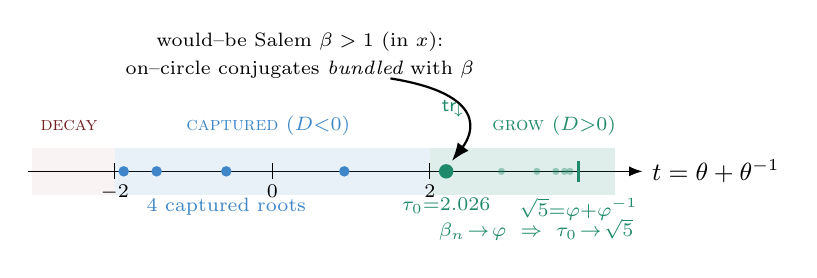
\begin{tikzpicture}[x=1cm,y=1cm,>=Latex]
\draw[->] (-3.1,0)--(4.7,0) node[right]{\small $t=\theta+\theta^{-1}$};
\fill[capc,opacity=.12]  (-2,-.30) rectangle (2,.30);
\fill[growc,opacity=.14] (2,-.30)  rectangle (4.35,.30);
\fill[openc,opacity=.06] (-3.05,-.30) rectangle (-2,.30);
\foreach \xp/\lab in {-2/$-2$,0/$0$,2/$2$}{\draw (\xp,-.10)--(\xp,.10); \node[below,inner sep=1.5pt] at (\xp,-.12){\scriptsize \lab};}
\node[openc!70!black] at (-2.58,.58){\scriptsize \textsc{decay}};
\node[capc]  at (-0.05,.58){\scriptsize \textsc{captured} ($D{<}0$)};
\node[growc] at (3.58,.58){\scriptsize \textsc{grow} ($D{>}0$)};
\foreach \xp in {-1.887,-1.469,-0.585,0.914}{\fill[capc] (\xp,0) circle (1.9pt);}
\fill[growc] (2.208,0) circle (2.6pt);
\draw[growc,line width=1pt] (3.888,-.13)--(3.888,.13);
\foreach \xp in {2.91,3.36,3.60,3.71,3.78}{\fill[growc,opacity=.4] (\xp,0) circle (1.3pt);}
\node[capc,below,inner sep=1.5pt]  at (-0.585,-.28){\scriptsize 4 captured roots};
\node[growc,below,inner sep=1.5pt] at (2.208,-.28){\scriptsize $\tau_0{=}2.026$};
\node[growc,below,inner sep=1.5pt] at (3.888,-.28){\scriptsize $\sqrt5{=}\varphi{+}\varphi^{-1}$};
\node[growc] at (3.35,-.74){\scriptsize $\beta_n\!\to\!\varphi\ \Rightarrow\ \tau_0\!\to\!\sqrt5$};
\node[align=center,inner sep=1.5pt] at (0.35,1.48){\scriptsize would--be Salem $\beta>1$ (in $x$):\\[-2pt]\scriptsize on--circle conjugates {\itshape bundled} with $\beta$};
\draw[->,line width=.8pt] (1.5,1.18) .. controls (2.75,.98) and (2.55,.48) .. (2.28,.13);
\node[growc,inner sep=1pt] at (2.30,.80){\scriptsize $\trace$};
\end{tikzpicture}
\caption{\small The trifurcation lives on the trace line, cut by the flip $t=\pm2$ ($t$ stretched $\times8$ beyond the flip). A would--be Salem is redirected by $\trace$ to $\tau_0=\beta+\beta^{-1}$ in \textcolor{growc}{\textsc{grow}}; its conjugates become \textcolor{capc}{\textsc{captured}} roots in $(-2,2)$. Shown: Lehmer's five trace roots. As $\beta\to\varphi$ the redirection $\to\sqrt5=\varphi+\varphi^{-1}$ (\S\ref{sec:goldenlimit}).}
\label{fig:trace}
\end{figure}

This is the positive characterization. Where a Salem would sit --- on--circle, possibly with measure near $1$ --- the system carries a totally real Perron number $\tau_0$ in \textsc{grow}, just past the flip, with minimal polynomial the Salem's trace--down; downstairs the on--circle conjugates are merely the captured roots $\tau_j\in(-2,2)$ of the same $T$ (Figure~\ref{fig:trace}).

\section{The action just past the flip: a branch point}\label{sec:flip}

Theorem~\ref{thm:occupant} places the occupant ``just past $t=2$.'' The structure there is governed by the fact that the flip is a \emph{branch point} of the two--to--one cover $t\mapsto x$.

\begin{lemma}[Square--root edge]\label{lem:sqrtedge}
The grow root $\beta(t)=\tfrac12\bigl(t+\sqrt{t^2-4}\bigr)$ satisfies, as $t\to2^+$,
\[
\beta(t)\ =\ 1+\sqrt{t-2}+\tfrac12(t-2)+\tfrac18(t-2)^{3/2}+O\!\bigl((t-2)^{2}\bigr),
\qquad\text{so}\quad \beta(t)-1\ \sim\ \sqrt{t-2}.
\]
The cover is $\sqrt{\,}$--ramified at the flip; the grow channel switches on with a square--root edge, and the growth rate satisfies $\log\beta\sim\beta-1\sim\sqrt{t-2}$. \forced{} {\small(series expansion, \S\ref{sec:ledger})}
\end{lemma}

\begin{proposition}[Quadratic redirection near the floor]\label{prop:quad}
For every $\beta>1$,
\[
\tau_0-2\ =\ \frac{(\beta-1)^2}{\beta}\qquad\text{exactly.}
\]
A Salem of height $\beta=1+\delta$ is therefore redirected to $\tau_0=2+\dfrac{\delta^2}{1+\delta}=2+\delta^2+O(\delta^3)$: only $\delta^2$ past the flip. \forced
\end{proposition}
\begin{proof}
$\beta+\beta^{-1}-2=(\beta^2-2\beta+1)/\beta=(\beta-1)^2/\beta$.
\end{proof}

Lemma~\ref{lem:sqrtedge} and Proposition~\ref{prop:quad} are two readings of the same ramification: the height $\beta-1$ moves like $\sqrt{t-2}$ going up, equivalently the trace $\tau_0-2$ moves like $(\beta-1)^2$ coming down. For Lehmer, $\beta-1=0.176281$ gives $\tau_0-2=(\beta-1)^2/\beta=0.026418$, matching the computed trace exactly. The smaller the Salem, the more tightly its redirection hugs the flip; the branch point is where the redirected outputs are most compressed ($d\beta/d\tau_0=(1-\beta^{-2})^{-1}\to\infty$ as $\beta\to1^+$), which is why the interesting action concentrates ``just past $t=2$.''

\begin{figure}[t]
\centering
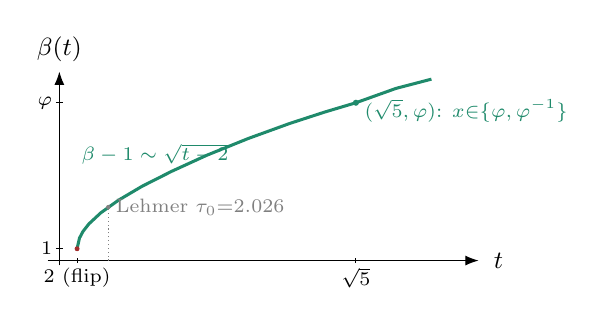
\begin{tikzpicture}[x=15cm,y=3.0cm,>=Latex]
% axes (t from 1.98..2.32 ; beta 0.95..1.72)
\draw[->] (1.975,0.95)--(2.34,0.95) node[right,xshift=2pt]{\small $t$};
\draw[->] (1.985,0.93)--(1.985,1.75) node[above]{\small $\beta(t)$};
% ticks
\draw (2,0.94)--(2,0.96); \node[below,inner sep=2pt] at (2,0.945){\scriptsize $2$ (flip)};
\draw (2.236068,0.94)--(2.236068,0.96); \node[below,inner sep=2pt] at (2.236068,0.945){\scriptsize $\sqrt5$};
\draw (1.982,1.0)--(1.988,1.0); \node[left,inner sep=2pt] at (1.984,1.0){\scriptsize $1$};
\draw (1.982,1.618034)--(1.988,1.618034); \node[left,inner sep=2pt] at (1.984,1.618034){\scriptsize $\varphi$};
% the curve beta(t)=(t+sqrt(t^2-4))/2
\draw[growc,line width=1.1pt] plot coordinates {
(2.000,1.00000)(2.002,1.04480)(2.005,1.07326)(2.010,1.10512)(2.020,1.15178)
(2.035,1.20536)(2.055,1.26430)(2.080,1.32757)(2.110,1.39616)(2.145,1.46686)
(2.180,1.53033)(2.210,1.57920)(2.236068,1.61803)(2.270,1.67877)(2.300,1.71789)};
% mark flip and golden landing
\fill[openc] (2,1.0) circle (.9pt);
\fill[growc] (2.236068,1.618034) circle (1.1pt);
\node[growc,right,inner sep=3pt] at (2.236068,1.585){\scriptsize $(\sqrt5,\varphi)$: $x{\in}\{\varphi,\varphi^{-1}\}$};
% Lehmer tau0 marker
\draw[densely dotted,gray] (2.026418,0.95)--(2.026418,1.176281);
\fill[gray] (2.026418,1.176281) circle (.8pt);
\node[gray,right,inner sep=2.5pt] at (2.0265,1.176){\scriptsize Lehmer $\tau_0{=}2.026$};
% sqrt edge annotation
\node[growc,align=left] at (2.066,1.40){\scriptsize $\beta-1\sim\sqrt{t-2}$};
\end{tikzpicture}
\caption{\small The grow root $\beta(t)=\tfrac12(t+\sqrt{t^2-4})$ on the grow side of the flip. The square--root edge at $t=2$ (vertical tangent) is the branch point: $\beta-1\sim\sqrt{t-2}$. The interval $(2,\sqrt5\,]$ in trace corresponds to real pairs $\{\beta,\beta^{-1}\}$ with $\beta\in(1,\varphi]$; the endpoint $t=\sqrt5$ lifts to the golden pair $\{\varphi,\varphi^{-1}\}$. Lehmer's redirection $\tau_0=2.026$ sits just past the flip.}
\label{fig:edge}
\end{figure}

\begin{lemma}[{The interval $(2,\sqrt5\,]$ and its lift}]\label{lem:interval}
The endpoints lift as $t=2\mapsto x=1$ (the degenerate root of unity, the captured/grow boundary) and $t=\sqrt5\mapsto x^2-\sqrt5\,x+1=0$, i.e.\ $x\in\{\varphi,\varphi^{-1}\}$. Since $\trace$ is strictly increasing on $\beta>1$, the grow interval $(2,\sqrt5\,]$ is exactly $\trace\bigl((1,\varphi]\bigr)$: the traces of the real pairs $\{\beta,\beta^{-1}\}$ with $\beta$ from $1$ up to the golden ratio. \forced
\end{lemma}

Thus the sub--floor Salem range $\beta\in(1,\varphi)$ --- precisely the heights that would breach the cost floor --- is mapped by $\trace$ \emph{onto} the open interval $(2,\sqrt5)$, bounded above by $\sqrt5$. The golden floor $\beta=\varphi$ is the supremum, with image $\sqrt5$ (Figure~\ref{fig:edge}). The next section shows that value is reached in the limit and identifies it.

\section{What it does instead: real growth for on--circle structure}\label{sec:does}

The redirected object is not a passive placeholder; it carries strictly more growth than the Salem it replaces, and it does so by re--sorting, not destroying, the on--circle data.

\begin{corollary}[The entropy trade]\label{cor:entropy}
For every Salem $\beta$, $\ \log\Mah(T)\ge\log\tau_0=\log(\beta+\beta^{-1})>\log\beta=\log\Mah(\beta)$. \forced
\end{corollary}

\begin{remark}[What the trace map actually loses]\label{rem:loses}
The redirection does not annihilate the angles; it freezes them. Each on--circle conjugate $e^{\pm i\psi}$ of the Salem maps to the \textsc{captured} coordinate $2\cos\psi\in(-2,2)$, a root of $T$. Because $e^{i\psi}$ and $e^{-i\psi}$ share $2\cos\psi$, the \emph{only} datum discarded is orientation --- the sign of $\psi$. Growth goes to $\tau_0$ (\textsc{grow}); angle goes to $2\cos\psi$ (\textsc{captured}); nothing else is lost. The trace--down $T$ records both, sorted one--and--the--rest by the flip.
\end{remark}

The benchmark Salem numbers make the trade concrete (full data in \S\ref{sec:ledger}):
\begin{center}
\renewcommand{\arraystretch}{1.15}
\begin{tabular}{@{}lccccc@{}}
\toprule
Salem $\beta$ & $\Mah(\beta)=\beta$ & trace--down $T(t)$ & $\tau_0$ & $\Mah(T)$ & $\log\beta\to\log\tau_0$\\
\midrule
Lehmer (deg $10$) & $1.1762808$ & $t^5{+}t^4{-}5t^3{-}5t^2{+}4t{+}3$ & $2.026418$ & $5.615601$ & $0.162\to0.706$\\
$\beta_4$ (deg $4$)& $1.7220838$ & $t^2-t-3$ & $2.302776$ & $3.000000$ & $0.544\to0.834$\\
deg $6$ Salem & $1.5061357$ & $t^3-t^2-3t+1$ & $2.170086$ & $3.214320$ & $0.410\to0.775$\\
\bottomrule
\end{tabular}
\end{center}

\section{The golden limit and its rate}\label{sec:goldenlimit}

The previous sections are general. The next fact is specific to the golden system and is the reason the redirection closes the loop with the self--action.

\begin{lemma}[Golden trace identity]\label{lem:goldentrace}
$\varphi+\varphi^{-1}=\sqrt5$. \forced
\end{lemma}
\begin{proof}
$\varphi=\tfrac{1+\sqrt5}2$, $\varphi^{-1}=\varphi-1=\tfrac{\sqrt5-1}2$; sum $=\sqrt5$.
\end{proof}

\begin{theorem}[Redirection at the floor]\label{thm:goldenlimit}
Let $\{\beta_n\}$ be Salem numbers with $\beta_n\to\varphi$ (e.g.\ the Salem factors of $S_n=x^nP-P^*$, $P=x^2-x-1$, which approach $\varphi$ from below). Then
\[
\tau_0(\beta_n)=\beta_n+\beta_n^{-1}\ \longrightarrow\ \varphi+\varphi^{-1}=\sqrt5=+\sqrt D\in\spec(\ad_R).
\]
The slot at the golden floor is filled by $\sqrt5$, the $+\sqrt D$ generator of \textsc{grow}. \forced{} {\small(\texttt{P2-UNIF-01}; \S\ref{sec:ledger})}
\end{theorem}
\begin{proof}
$\trace$ is continuous on $\theta>1$, so $\beta_n\to\varphi$ gives $\tau_0\to\varphi+\varphi^{-1}=\sqrt5$. For the golden seed $\ad_R$ has eigenvalues the differences of $\varphi,\psi$, namely $\{0,\pm\sqrt5\}$, so $\sqrt5=+\sqrt D$.
\end{proof}

\paragraph{The rate.} The convergence has a clean two--fold description: first order in the height gap, geometric along the family.

\begin{proposition}[Linear rate, slope $\varphi^{-1}$]\label{prop:linrate}
$\trace'(\beta)=1-\beta^{-2}$, and $\trace'(\varphi)=1-\varphi^{-2}=\tfrac{\sqrt5-1}2=\varphi^{-1}$. Hence
\[
\sqrt5-\tau_0(\beta)\ =\ \varphi^{-1}(\varphi-\beta)\ -\ (\sqrt5-2)\,(\varphi-\beta)^2\ +\ O\!\bigl((\varphi-\beta)^3\bigr),
\]
the curvature coefficient being $\tfrac12\trace''(\varphi)=\sqrt5-2=\varphi^{-3}$. The approach is linear with slope $\varphi^{-1}$. \forced
\end{proposition}

\begin{theorem}[Geometric rate along the canonical family]\label{thm:georate}
For the Salem factors $\beta_n\to\varphi$ of $S_n=x^nP-P^*$, $P=x^2-x-1$,
\[
\varphi-\beta_n\ \sim\ \frac{2}{\sqrt5}\,\varphi^{\,1-n},
\qquad
\sqrt5-\tau_0(\beta_n)\ \sim\ \frac{2}{\sqrt5}\,\varphi^{-n},
\]
so consecutive gaps shrink by the factor $\varphi$ exactly. \computed{} {\small(verified $n\le29$, \S\ref{sec:ledger})}
\end{theorem}
\begin{proof}[Proof sketch]
At a Salem root, $\beta_n^{\,n}P(\beta_n)=P^*(\beta_n)$. With $P^*(x)=x^2P(1/x)=1-x-x^2$, one has $P^*(\varphi)=-2\varphi$ and $P'(\varphi)=2\varphi-1=\sqrt5$. Near $\varphi$, $P(\beta_n)\approx\sqrt5\,(\beta_n-\varphi)$ and $\beta_n^{\,n}\approx\varphi^n$, so $\varphi^n\sqrt5(\beta_n-\varphi)\approx-2\varphi$, giving $\varphi-\beta_n\approx(2/\sqrt5)\varphi^{1-n}$. Apply Proposition~\ref{prop:linrate}: $\sqrt5-\tau_0\approx\varphi^{-1}(\varphi-\beta_n)\approx(2/\sqrt5)\varphi^{-n}$.
\end{proof}

\begin{center}
\renewcommand{\arraystretch}{1.15}
\begin{tabular}{@{}rccc@{}}
\toprule
$n$ & $\sqrt5-\tau_0(\beta_n)$ & $(\sqrt5-\tau_0)\cdot\varphi^{\,n}$ & consecutive ratio\\
\midrule
$9$  & $1.289085\times10^{-2}$ & $0.979875$ & $1.68711$\\
$12$ & $2.858434\times10^{-3}$ & $0.920407$ & $1.64037$\\
$15$ & $6.613990\times10^{-4}$ & $0.902149$ & $1.62501$\\
$18$ & $1.551834\times10^{-4}$ & $0.896649$ & $1.62012$\\
$21$ & $3.656841\times10^{-5}$ & $0.895048$ & $1.61863$\\
$24$ & $8.628276\times10^{-6}$ & $0.894597$ & $1.61820$\\
$27$ & $2.036577\times10^{-6}$ & $0.894473$ & $1.61808$\\
\midrule
limit & --- & $2/\sqrt5=0.894427$ & $\varphi=1.618034$\\
\bottomrule
\end{tabular}
\end{center}

\begin{remark}[The channel--spectral form, completed]\label{rem:closed}
The companion papers note that the gap endpoints in the four domains --- height $\varphi$, entropy $\log\varphi$, channel threshold $\sqrt5$ --- are tied by structure, not a shared number. Theorem~\ref{thm:goldenlimit} supplies the arrow: $\trace$ maps the height datum to the channel datum, $\trace(\varphi)=\sqrt5$, and Theorem~\ref{thm:georate} times it at rate $\varphi^{-n}$. The would--be fourth channel at the floor is occupied by the image of the floor under the system's own decision map.
\end{remark}

\section{The redirection is forced, not chosen}\label{sec:forced}

One step above deserves scrutiny: the claim that the trace--down is what the system \emph{produces}, rather than a natural map an analyst chose. It is forced, by an identity the seed already satisfies.

\begin{proposition}[Trace map $=$ self--action grow eigenvalue]\label{prop:forced}
Let the seed be $x^2-ax-1$ $(a\ge1)$, with roots $\varphi_a>1>0>\psi_a$. Its constant term $-1$ forces $\varphi_a\psi_a=-1$, i.e.\ the conjugate is the negative reciprocal, $\psi_a=-\varphi_a^{-1}$. Then the grow eigenvalue of $\ad_R$ and the trace--down of the dominant root coincide:
\[
\underbrace{\varphi_a-\psi_a}_{\text{$\ad_R$ grow eigenvalue}}\ =\ \varphi_a+\varphi_a^{-1}\ =\ \underbrace{\trace(\varphi_a)}_{\text{trace--down}}\ =\ \sqrt{a^2+4}.
\]
For the golden seed $a=1$ this is $\sqrt5=+\sqrt D$. \forced
\end{proposition}
\begin{proof}
$\psi_a=-\varphi_a^{-1}$ gives $\varphi_a-\psi_a=\varphi_a+\varphi_a^{-1}$; both equal $\sqrt{a^2+4}$ by the quadratic formula.
\end{proof}

So $\theta\mapsto\theta+\theta^{-1}$ is not imported. Because the seed's conjugate is the negative reciprocal (a unit of norm $-1$), the trace map \emph{is} the operation computing the self--action's grow eigenvalue. Two consequences follow. First, the trace--down is the system's native coordinate twice over: it is the flip coordinate in which Salem is \emph{defined} (\emph{Emission--Gap}, \S on the flip), and it is the map producing $\spec(\ad_R)$'s grow value. Reading a would--be Salem in that coordinate returns $\tau_0$ in \textsc{grow} unambiguously. Second, the residual interpretive content shrinks to a naming choice: whether to call $\tau_0$ what the system ``produces'' or what its coordinate ``represents.'' Mathematically the object is fixed --- the system never forms the Salem upstairs, and downstairs the object is $T$ with dominant root $\tau_0$. The map carrying the one to the other is the system's own.

\section{Other occupants: the Pisot--trace accumulation}\label{sec:others}

The family limit $\sqrt5$ is one point; the slot has more structure.

\begin{proposition}[Accumulation points are Pisot traces]\label{prop:pisot}
By Salem's theorem every Pisot number $\theta$ is a two--sided limit of Salem numbers; since $\trace$ is continuous, the values $\{\tau_0(\beta):\beta\ \text{Salem}\}$ accumulate at $\{\theta+\theta^{-1}:\theta\ \text{Pisot}\}$. As $\varphi$ is the least limit point of the Pisot set, $\sqrt5=\trace(\varphi)$ is the least such trace--accumulation. The smallest Pisot number, the plastic number $\mu_P\approx1.324718$ (root of $x^3-x-1$), contributes the accumulation $\mu_P+\mu_P^{-1}\approx2.079596$. \computed{} {\small(plastic family verified, \S\ref{sec:ledger})}
\end{proposition}

The picture is therefore layered. Individual Salems map to individual points $\tau_0>2$ (the redirection is injective, since $\trace$ is strictly increasing). These points cluster at the Pisot traces, and those clusters themselves begin at $\sqrt5$ --- the golden value --- because $\varphi$ is where the Pisot set first accumulates. The appearance of $\sqrt5$ at the floor is not an isolated coincidence but the smallest instance of a general phenomenon, singled out because the golden seed sits exactly at the least Pisot limit point.

\section{Stress-testing the entry: the slot is a superselection sector}\label{sec:entry}

Sections~\ref{sec:redirect}--\ref{sec:goldenlimit} answered where a would--be occupant is \emph{sent}. The sharper question is dual: can anything \emph{enter}? If some construction --- linear or not --- could land an object in the slot, the slot would be a fillable void and the redirection merely its preferred exit. If none can, the slot is a different object: a region that \emph{rejects} filling. We stress--test every entry route we can make precise and find the second.

\begin{definition}[Entry map and conserved charge]\label{def:entry}
The \emph{lift} of a totally real $T\in\Z[t]$ is $L(T)(x)=x^{\deg T}\,T(x+x^{-1})\in\Z[x]$, a reciprocal polynomial; it is the inverse of the trace--down --- the only way to assemble an on--circle--plus--expanding object from a trace. For $P\in\Z[x]$ let the \emph{angle charge}
\[
A(P)=1 \iff \text{every root of }P\text{ has argument in }\tfrac\pi2\Z=\{0,\tfrac\pi2,\pi,\tfrac{3\pi}2\},
\]
and the \emph{Kronecker charge} $Q(P)=1$ iff every on--circle root of $P$ is a root of unity. An on--circle root with argument in $\tfrac\pi2\Z$ is a fourth root of unity, so $A=1\Rightarrow Q=1$.
\end{definition}

\begin{proposition}[Emittable $\Rightarrow A=1$; Salem $\Rightarrow A=0$]\label{prop:charge}
Every catalog generator has all roots at arguments in $\tfrac\pi2\Z$: the real seeds at $\{0,\pi\}$, and $K=x^4+5x^2-5$ with its imaginary pair $\pm i\beta$ at $\pm\tfrac\pi2$. Hence $A=1$, preserved by the operators (Theorem~\ref{thm:superselect}). A Salem number has an on--circle conjugate at an irrational multiple of $\pi$ --- else its minimal polynomial is cyclotomic and $\beta$ a root of unity --- so $A=0$ and $Q=0$. The Salem slot is exactly $\{A=0\ \wedge\ \text{expanding}\}$. \computed{} {\small(\S\ref{sec:ledger}: $\varphi{\otimes}\varphi$ has on--circle root $-1$ of order $2$; $\varphi^4{\otimes}\varphi^4$ has $+1$ of order $1$)}
\end{proposition}

\begin{theorem}[Superselection: no operation changes the charge]\label{thm:superselect}
The emission operators preserve $A=1$, so none maps the $A=1$ sector into the $A=0$ slot:
\begin{itemize}[leftmargin=1.5em,itemsep=1pt]
\item $\oplus$ unions the root multisets, and $\tfrac\pi2\Z$ is closed under union;
\item $(\cdot)^2$ doubles arguments, and $2\cdot\tfrac\pi2\Z\subseteq\tfrac\pi2\Z$;
\item $\otimes$ adds arguments ($\arg\lambda\mu=\arg\lambda+\arg\mu$), and $\tfrac\pi2\Z+\tfrac\pi2\Z\subseteq\tfrac\pi2\Z$.
\end{itemize}
Thus $A$ is a conserved charge of the emission algebra and the slot is a forbidden superselection sector. \forced
\end{theorem}
\begin{proof}
The three closures are immediate; composition of charge--preserving maps preserves the charge. A root of unity has rational argument, in $\tfrac\pi2\Z$ for the reachable angles; an irrational--angle Salem conjugate is not in the image of any finite word in the operators.
\end{proof}

\begin{center}
\renewcommand{\arraystretch}{1.22}
\begin{tabular}{@{}p{0.27\linewidth} p{0.34\linewidth} p{0.15\linewidth} c@{}}
\toprule
entry route & mechanism & effect on $A$ & reaches slot? \\
\midrule
trace lift $L$ (linear) & $x^2-tx+1$; lattice $t\in\{-2,0,2\}\to$ roots of unity & preserves $A{=}1$ & no (reducible)\\
direct sum $\oplus$ (superposition) & union of spectra & preserves $A{=}1$ & no\\
block--diagonal (suspended superposition) & captured $\oplus$ grow & preserves $A{=}1$, reducible & no\\
monodromy / curvature (non--linear travel) & permutes $\{\beta,\beta^{-1}\}$ around the branch point $t{=}2$ & preserves $A$ (same root set) & no\\
free commutator $[A,B]$ & off--diagonal coupling & breaks the field & not an operation\\
limit (Salem's theorem) & Pisot $\to$ Salem accumulation & $A{=}1\to A{=}0$ \emph{in the limit} & approached, never attained\\
\bottomrule
\end{tabular}
\end{center}

\paragraph{The lift is innocent on the lattice.} The lift of a lattice captured position is a root of unity:
\[
L(t{=}2)=x^2-2x+1=(x-1)^2,\quad L(0)=x^2+1,\quad L(-2)=(x+1)^2 .
\]
Only an \emph{off--lattice} captured position $2\cos\psi$ with $\psi/\pi$ irrational lifts to a Salem conjugate (for $\beta_4$, the trace root $\tfrac{1-\sqrt{13}}2=-1.3028$ lifts to its conjugate at $0.726\pi$). Emittable trace--downs have their captured roots pinned to $\{-2,0,2\}$ (Proposition~\ref{prop:charge}), so $L$ applied to anything the algebra produces is reducible --- cyclotomic times grow --- never a Salem.

\paragraph{Superposition and its suspension.} Direct sum \emph{is} superposition of spectra; it keeps $A=1$. A ``suspended'' superposition --- the two channels held without collapse --- is a block--diagonal $\textsc{captured}\oplus\textsc{grow}$, hence reducible: $(-1)\oplus(x^2-3x+1)=(x+1)(x^2-3x+1)$, and indeed $\varphi\otimes\varphi=(x+1)^2(x^2-3x+1)$ is exactly this form. To fuse the blocks into one \emph{irreducible} Salem requires an off--diagonal coupling; the structure--preserving couplings keep it reducible, and a generic coupling is the free commutator $[A,B]$, which leaves $\Z[x]$ and breaks the field --- the operation the construction names as foreign to itself. Superposition cannot cross the sector boundary; that is the content of ``superselection.''

\paragraph{Non--linear travel is monodromy.} A curved or non--linear path is, for the algebraic data, a closed loop in parameter space, and its only action is the monodromy permutation of roots. Around the branch point $t=2$, analytic continuation of $\beta(t)=\tfrac12(t+\sqrt{t^2-4})$ once returns $\beta\mapsto\beta^{-1}$ (verified: $\beta=1.71789$ at $t=2.3$ returns as $0.58211=\beta^{-1}$). The orbit is $\{\beta,\beta^{-1}\}$ --- the two roots of the same quadratic. Curvature reshuffles existing roots; it never bundles emittable pieces into a new irreducible Salem.

\paragraph{The one frontier: limits.} Salem's theorem makes every Salem number a two--sided limit of Pisot numbers, and the catalog \emph{has} Pisot generators $\varphi,\varphi^4$. This is the single route by which $A=0$ is approached. But it is not an operation: the emission algebra is finitely generated, its Mahler spectrum a discrete sub--semigroup of $[\varphi,\infty)$ with no accumulation at $1$ (companion paper, Rem.~``finitely generated''). The sub--$\varphi$ Salem band $(1,\varphi)$ is disjoint from the image; the boundary is approached and never reached.

\begin{theorem}[The slot rejects filling]\label{thm:rejects}
No emission operation --- $\oplus$, $\otimes$, squaring, the lift $L$, their finite compositions, or the monodromy of any closed parameter path --- carries an emittable object into the Salem slot, because every such operation preserves the angle charge $A$ (Theorem~\ref{thm:superselect}) while the slot has $A=0$. The only route to $A=0$ is a limit, which the finitely generated algebra approaches but never attains. The slot is therefore not a void that can be filled but a \emph{space that rejects filling}, coincident with the limit frontier of the emittable set --- reached by nothing inside it. \forced
\end{theorem}

This resolves the dichotomy. The ``would--be occupant'' of \S\S\ref{sec:redirect}--\ref{sec:goldenlimit} is exactly that: a hypothetical the charge $A$ forbids on entry and the trace projection $\trace$ expels on contact. Entry is impossible (superselection), exit is forced ($\beta\mapsto\beta+\beta^{-1}$ into \textsc{grow}), and the value the exit accumulates at is $\sqrt5$, the grow generator. The slot is empty not by accident of the current generating set but by a conservation law: the angle charge is the system's superselection rule, and the Salem regime is the sector it cannot enter.


\section{The upstairs shadow: cyclotomic times grow}\label{sec:upstairs}

Downstairs the redirection is the trace map. Upstairs the same fact is a forced factorization, exhibited by the construction that manufactures Salem numbers.

\begin{proposition}[Forcing the lattice breaks irreducibility]\label{prop:factor}
If a reciprocal $P\in\Z[x]$ has all on--circle roots at fourth roots of unity, then $P$ is divisible by a cyclotomic polynomial; an irreducible Salem polynomial (on--circle conjugates at irrational angle) therefore has none. When on--circle structure is forced onto the lattice the object splits as cyclotomic $(\textsc{captured},\ \Mah=1)$ times real reciprocal $(\textsc{grow},\ \Mah\ge\varphi)$. \forced{} {\small(\texttt{P2-ANG-03/04})}
\end{proposition}

The construction $S_n(x)=x^nP(x)-P^*(x)$, $P=x^2-x-1$, displays the split: its non--cyclotomic factor is a Salem climbing to $\varphi$, the cyclotomic remainder the \textsc{captured} cloud.
\begin{center}
\renewcommand{\arraystretch}{1.15}
\begin{tabular}{@{}cll@{}}
\toprule
$n$ & factorization of $S_n$ & channels\\
\midrule
$6$ & $(x-1)(x+1)\,(x^6-x^5-x^3-x+1)$ & \textsc{captured}$\times$\textsc{grow}, $\Mah=1.5061$\\
$10$& $(x-1)(x+1)(x^2{+}x{+}1)\,(x^8{-}2x^7{+}x^6{-}x^4{+}x^2{-}2x{+}1)$ & \textsc{captured}$\times$\textsc{grow}, $\Mah=1.6054$\\
$12$& $(x-1)(x+1)\,(x^{12}{-}x^{11}{-}x^9{-}x^7{-}x^5{-}x^3{-}x{+}1)$ & \textsc{captured}$\times$\textsc{grow}, $\Mah=1.6134$\\
\bottomrule
\end{tabular}
\end{center}
Upstairs the would--be Salem is a product across the two existing channels; downstairs that product is the single totally real trace--down whose dominant root is the \textsc{grow} occupant of Theorem~\ref{thm:occupant}.

\section{Epistemic ledger}\label{sec:ledger}

\begin{center}
\renewcommand{\arraystretch}{1.16}
\begin{tabular}{@{}p{8.0cm}cl@{}}
\toprule
\textbf{Claim} & \textbf{Status} & \textbf{Backing} \\
\midrule
Trace map sorts onto three regions; no fourth channel & \forced & Lem.~\ref{lem:regions}, Cor.~\ref{cor:nofourth}\\
$\tau_0=\beta+\beta^{-1}>2$ (AM--GM) & \forced & Lem.~\ref{lem:amgm}\\
Redirected $\Mah(T)\ge\tau_0>2>\varphi$, all Salem & \forced & Thm.~\ref{thm:occupant}\\
Flip is a branch point: $\beta-1\sim\sqrt{t-2}$ & \forced & Lem.~\ref{lem:sqrtedge}\\
$\tau_0-2=(\beta-1)^2/\beta$ exactly; near floor $\tau_0\approx2+\delta^2$ & \forced & Prop.~\ref{prop:quad}\\
$t{=}2\mapsto x{=}1$; $t{=}\sqrt5\mapsto\{\varphi,\varphi^{-1}\}$; $(2,\sqrt5]=\trace((1,\varphi])$ & \forced & Lem.~\ref{lem:interval}\\
Entropy trade $\log\tau_0>\log\beta$; angle frozen to $2\cos\psi$ & \forced & Cor.~\ref{cor:entropy}, Rem.~\ref{rem:loses}\\
$\varphi+\varphi^{-1}=\sqrt5$; $\beta_n\!\to\!\varphi\Rightarrow\tau_0\!\to\!\sqrt5\in\spec(\ad_R)$ & \forced & Lem.~\ref{lem:goldentrace}, Thm.~\ref{thm:goldenlimit}\\
Linear rate slope $\trace'(\varphi)=\varphi^{-1}$; curvature $\sqrt5-2=\varphi^{-3}$ & \forced & Prop.~\ref{prop:linrate}\\
Geometric rate $\sqrt5-\tau_0\sim(2/\sqrt5)\varphi^{-n}$, ratio $\to\varphi$ & \computed & Thm.~\ref{thm:georate}; table, $n\le29$\\
Lehmer $\tau_0{=}2.026418$, $\Mah(T){=}5.615601$ & \computed & \S\ref{sec:does}\\
Trace map $=$ $\ad_R$ grow eigenvalue ($\varphi\psi{=}-1$) & \forced & Prop.~\ref{prop:forced}\\
Accumulations $=$ Pisot traces; $\sqrt5$ least; plastic $\to2.0796$ & \computed & Prop.~\ref{prop:pisot}\\
Lattice forcing $\Rightarrow$ cyclotomic $\times$ grow; $S_n$ exhibits it & \forced & Prop.~\ref{prop:factor}\\
Emittable root angles confined to $\tfrac\pi2\Z$ (charge $A{=}1$) & \computed & Prop.~\ref{prop:charge}\\
Superselection: $\oplus,\otimes,(\cdot)^2$ preserve $A$; slot has $A{=}0$ & \forced & Thm.~\ref{thm:superselect}\\
Lift of lattice $\{-2,0,2\}$ = roots of unity; off--lattice = Salem conj. & \forced & \S\ref{sec:entry}\\
Monodromy round $t{=}2$ swaps $\beta\leftrightarrow\beta^{-1}$, no new object & \computed & \S\ref{sec:entry}\\
Slot rejects filling; only limits approach (never attain) & \forced & Thm.~\ref{thm:rejects}\\
\bottomrule
\end{tabular}
\end{center}

\paragraph{Summary.} When a construction drifts toward the Salem slot, the system carries the trace redirection $\tau_0=\beta+\beta^{-1}$: a totally real Perron number in \textsc{grow}, lodged just past the flip --- a square--root branch point at which the channel switches on, so a Salem of height $1{+}\delta$ lands only $\delta^2$ past $t=2$. Its measure is forced above the floor, its growth strictly exceeds the Salem's, and the on--circle data is not destroyed but frozen into captured coordinates $2\cos\psi$. As Salems climb to the golden floor the occupant converges to $\sqrt5=\varphi+\varphi^{-1}$ --- the grow generator of $\ad_R$ --- linearly with slope $\varphi^{-1}$ and geometrically at rate $\varphi^{-n}$ along the canonical family. That the trace map is the right map is not a modeling choice: because the seed conjugate is the negative reciprocal, the trace map is exactly the operation computing the self--action's grow eigenvalue. And $\sqrt5$ at the floor is the smallest instance of a general layering --- Salem redirections cluster at the Pisot traces, which begin at $\varphi$. Where the companion papers proved Salem \emph{absent}, this note names what is \emph{present}, locates it to a branch point, times its approach, and shows the map that puts it there is the system's own.

\end{document}
